\documentclass[12pt]{article}
\usepackage{parskip}
\usepackage{amsmath}
\usepackage{pdfpages}
\usepackage{listings}
\usepackage{color}
\usepackage[margin=.6in]{geometry}

\definecolor{dkgreen}{rgb}{0,0.6,0}
\definecolor{gray}{rgb}{0.5,0.5,0.5}
\definecolor{mauve}{rgb}{0.58,0,0.82}

\lstset{frame=tb,
  language=C++,
  aboveskip=3mm,
  belowskip=3mm,
  showstringspaces=false,
  columns=flexible,
  basicstyle={\small\ttfamily},
  numbers=none,
  numberstyle=\tiny\color{gray},
  keywordstyle=\color{blue},
  commentstyle=\color{dkgreen},
  stringstyle=\color{mauve},
  breaklines=true,
  breakatwhitespace=true,
  tabsize=3
}


\begin{document}
\includepdf[pages=5]{slides.pdf} 
Think Taboo (dunno why its spelt wrong, but it is). You remember as you go so that you dont repeat looking at things. If you have found something better, never come back to this solution. Maintain a taboo list that you put things in as you go since they are worse than you did. You can relook at the taboo list if you hit a stop point that doesn't work.

\includepdf[pages=6]{slides.pdf} 
This is basically what you thought hill climbing was.

\includepdf[pages=7-9]{slides.pdf} 
A problem to consider is how far back your memory should go. We can also note solutions that are frequently chosen as they are probably pretty good.

\includepdf[pages=10-21]{slides.pdf} 
In this example you can try switching around the order of filters. You evaluate if this solution improves everything. One approach is to enumerate all solutions and evaluate which is best. This can be costly though. 

\includepdf[pages=22]{slides.pdf} 
From this solution we have to move somewhere. What is a move? Well we could do stuff like swapping things around. 

\includepdf[pages=23-24]{slides.pdf} 
There are a tone of different arrangements you can have. With this it is not really feasible. We have to just ignore some possibilities. The most optimal solution may be in there but we are still going to improve our algorithm.

\includepdf[pages=25-27]{slides.pdf} 
We can define the memory of the tabu as the number of parameters to be considered. Here we only classify the three most recent solutions as tabu.


IGNORE HIS EXAMPLE, GOOGLE HOW TABU ALGORITHMS WORK

\includepdf[pages=35-36]{slides.pdf} 
One thing you have to do is vary the tabu size (between and min and max) to see how if effects the solution chosen. We want to make sure that we don't have cycles, but we still want to limit the memory used. Gotta find some happy medium.

\includepdf[pages=37-38]{slides.pdf} 
Intensification is when we keep incrementally improving the current solution by exploring neighborhoods that are promissing. When this stagnates we go to some random area and hope for the the best (called diversification).

\includepdf[pages=39-44]{slides.pdf} 
The 8 queens problem is a common problem to think about. Basically put 8 queens on the board such that none of them can take each other. We evaluate a solution by the number of collisions between queens that can happen. We can make a move by swapping rows.

\includepdf[pages=72]{slides.pdf} 
THIS IS TERRIBLY EXPLAINED GOOGLE WHAT THE FUCK THIS GUY IS TALKING ABOUT.  

\end{document}